\chapter{Path Integrals for Interacting Complex Scalar Fields}
\section{The complex scalar field}
\subsection{Lagrangian, equations of motion, conjugate momenta and Hamiltonian}
So far we have worked solely with the real scalar field. Now we consider the Lagrangian density
\begin{equation}
\mathcal{L}=-\partial^{\mu} \phi^{\dagger} \partial_{\mu} \phi-{m}^{2} \phi^{\dagger} \phi+\Omega_{0}
\end{equation}
with the action being $S=\int\dd^4 x\, \mathcal{L}$. We treat $\phi$ and $\phi^\dagger$ as independent field variables and the equations of motion follow from the variational principle
\begin{equation}
    -\fdv{S}{\phi^\dagger}=-\pdv{\mathcal{L}}{\phi^\dagger}+\partial_\mu\pdv{\mathcal{L}}{(\partial_\mu\phi^\dagger)}=(-\partial^2+m^2)\phi=0
    \label{eom1}
\end{equation}
\begin{equation}
    -\fdv{S}{\phi}=-\pdv{\mathcal{L}}{\phi}+\partial_\mu\pdv{\mathcal{L}}{(\partial_\mu\phi)}=(-\partial^2+m^2)\phi^\dagger=0
    \label{eom2}
\end{equation}
so that both $\phi$ and $\phi^\dagger$ obey the Klein-Gordon equation. The conjugate momenta are
\begin{equation}
    \Pi(x)=\pdv{\mathcal{L}}{\dot{\phi}}=\dot{\phi}^\dagger
\end{equation}
\begin{equation}
    \Pi^\dagger(x)=\pdv{\mathcal{L}}{\dot{\phi}^\dagger}=\dot{\phi}
\end{equation}
so the Hamiltonian density $\mathcal{H}=\Pi(x) \dot{\phi}+\Pi^{\dagger}(x) \dot{\phi}^{\dagger}-\mathcal{L}$ reads
\begin{equation}
\mathcal{H}=\Pi^{\dagger}(x) \Pi(x)+\nabla \phi^{\dagger} \nabla \phi+m^{2} \phi^{\dagger} \phi-\Omega_{0}.
\end{equation}
From equations (\ref{eom1}) and (\ref{eom2}), the following mode expansion arises as a solution
\begin{equation}
     \phi(x)=\int\widetilde{\dd k}\, [a(\vb{k})e^{ikx}+b^\dagger(\vb{k})e^{-ikx}].
\end{equation}
multiplying this mode expansion by exponentials and integrating over space allows us to find
\begin{equation}
a(\mathbf{k})=\int \dd^{3} x\, e^{-i k x}\left(\omega \phi(x)+i \partial_{0} \phi(x)\right)
\label{azinho}
\end{equation}
\begin{equation}
b(\mathbf{k})=\int \dd^{3}x\, e^{-i k x}\left(\omega \phi^\dagger(x)+i \partial_{0} \phi^\dagger(x)\right)
\label{bzinho}
\end{equation}
With $a^\dagger$ and $b^\dagger$ following from hermitian conjugation. The relevant commutation relations at equal times are
\begin{equation}
\begin{aligned}
\comm{\phi(x)}{\Pi(x^\prime)}&=i\delta^3(\vb{x}-\vb{x}^\prime)\\
\comm{\phi^\dagger(x)}{\Pi^\dagger(x^\prime)}&=i\delta^3(\vb{x}-\vb{x}^\prime)
\end{aligned}
\end{equation}
with other possible combinations between $\phi$, $\Pi$, $\phi^\dagger$ and $\Pi^\dagger$ vanishing. From (\ref{azinho}) and (\ref{bzinho}) and their conjugates, we can check that
\begin{equation}
    \begin{aligned}
    \comm{a(\vb{k})}{a^\dagger(\vb{k}^\prime)}&=(2\pi)^3 2\omega \delta^3(\vb{k}-\vb{k}^\prime)\\
    \comm{b(\vb{k})}{b^\dagger(\vb{k}^\prime)}&=(2\pi)^3 2\omega \delta^3(\vb{k}-\vb{k}^\prime)
    \end{aligned}
\end{equation}
with other combinations  vanishing. $a^\dagger(\vb{k})$ and $b^\dagger(\vb{k})$ and their conjugates are creation and annihilation operators. This highlights that, in the case of the complex field, there are two types of particles: those created by $b^\dagger$ and those created by $a^\dagger$ when they act on the vacuum state $\ket{0}$, assumed to be normalized $\braket{0}=1$ and to vanish upon the action of annihilation operators $a(\vb{k})\ket{0}=b(\vb{k})\ket{0}=0$ for any $\vb{k}$.\\

Expressing the total Hamiltonian in terms of the creation and annihilation operators gives
\begin{equation}
H=-\Omega_{0} V+\int \widetilde{d k}\,\omega\left[a^{\dagger}(\vb{k}) a(\vb{k})+b^{\dagger}(\vb{k}) b(\vb{k})+(2 \pi)^{3} 2 \omega \delta^{3}(\vb{0})\right].
\end{equation}
Interpreting $(2\pi)^3\delta^3(\vb{0})$ as the volume of space and integrating the last term up to a cutoff gives
\begin{equation}
    H=(2\mathcal{E}_0-\Omega_0)V+\int \widetilde{d k}\,\omega\left[a^{\dagger}(\vb{k}) a(\vb{k})+b^{\dagger}(\vb{k}) b(\vb{k})\right]
\end{equation}
where $\mathcal{E}_0=\frac{1}{2(2\pi)^3}\int\dd^3 k\,\omega$ integrated up to a cutoff $\Lambda$ is the zero point energy density of the oscillators. We set $\Omega_0=2\mathcal{E}_0$ to make the Hamiltonian ground state equal to zero.
\subsection{The LSZ formula for the complex scalar field}
Since there are two types of particles in a complex theory, we can have different combinations of types of particles  when preparing initial and final states for the $\braket{f}{i}$ amplitude.
%When there is only one kind of particle involved in both the initial and final states, we use the the LSZ formula we already derived. 
Following similar steps we took when deriving the LSZ for the first time, it is easy to show that the LSZ formula, for initial and final states with $a$- and $b$-type particles, for instance, reads
\begin{equation}
\begin{aligned}
        \braket{f}{i}&=\vev{\text{T}a_{1^\prime}(+\infty)b_{2^\prime}(+\infty)a^\dagger_1(-\infty)b^\dagger_2(-\infty)}\\
        &=i^4\int \dd^4x_1\dd^4x_2\dd^4x_{1^\prime}\dd^4x_{2^\prime}e^{ik_1x_1}e^{ik_2x_2}e^{-ik_1^\prime x_{1^\prime}}e^{-ik_2^\prime x_{2^\prime}}\\
        &\qquad\times(-\partial^2_{1}+m^2_{1})(-\partial^2_{2}+m^2_{2})(-\partial^2_{1^\prime}+m^2_{1^\prime})(-\partial^2_{2^\prime}+m^2_{2^\prime})\\
        &\qquad\times\vev{\text{T}\phi(x_{1^\prime})\phi^\dagger(x_{2^\prime})\phi^\dagger(x_1)\phi(x_2)}
\end{aligned}
\end{equation}
where $a_i^\dagger$ or $b_i^\dagger$ are the wave-packet creation operators in the interacting theory, where they pick-up time dependence but behave as the free theory operators do if the field satisfy  conditions that can be imposed via re-scaling and shifting the field, as we have seen in more detail in previous work. For different configurations of particles in the initial and final states, the following replacements into the vacuum expectation value readily give the LSZ.
\begin{equation}
    \begin{aligned}
    a_{1}^{\dagger}(-\infty)& \rightarrow i \int \dd^{4} x_{1}\, e^{+i k_{1} x_{1}}\qty(-\partial_{1}^{2}+m^{2}) \phi^{\dagger}\left(x_{1}\right),\\
    a_{1^{\prime}}(+\infty)& \rightarrow i \int \dd^{4} x_{1^{\prime}}\, e^{-i k_{1}^{\prime} x_{1^{\prime}}}\qty(-\partial_{1^{\prime}}^{2}+m^{2}) \phi(x_{1^{\prime}}),\\
    b_{2}^{\dagger}(-\infty)&\rightarrow i \int\dd^{4} x_{2}\, e^{+i k_{2} x_{2}}\qty(-\partial_{2}^{2}+m^{2}) \phi(x_{2}),\\
    b_{2^{\prime}}(+\infty)&\rightarrow i \int \dd^{4} x_{2^{\prime}}\, e^{-i k_{2}^{\prime} x_{2^{\prime}}}\qty(-\partial_{2^{\prime}}^{2}+m^{2}) \phi^{\dagger}(x_{2^{\prime}}).\\
    \end{aligned}
\end{equation}
\section{Path integral for the complex scalar field}
The presence of sources in the equations of motion for $\phi$ and $\phi^\dagger$ can be incorporated with the addition of $J^\dagger\phi+J\phi^\dagger$ to the action, so that the functional integral reads
\begin{equation}
    Z_0(J,J^\dagger)=\int\mathcal{D}\phi\exp[i\int\dd^4 x\,\qty(-\partial^\mu\phi^\dagger\partial_\mu\phi-m^2\phi^\dagger\phi+J^\dagger\phi+J\phi^\dagger)].
\end{equation}
Fourier transforming the fields and sources gives the action
\begin{equation}
S_{0}=\int \frac{d^{4} k}{(2 \pi)^{4}}\left[-\widetilde{\phi}^{\dagger}(k)\left(k^{2}+m^{2}\right) \widetilde{\phi}(k)+\widetilde{J}^{\dagger}(k) \widetilde{\phi}(k)+\widetilde{\phi}^{\dagger}(k) \widetilde{J}(k)\right]
\end{equation}
for which the translation 
\begin{equation}
\widetilde{\chi}=\widetilde{\phi}-\frac{\widetilde{J}(k)}{k^{2}+m^{2}}
\end{equation}
reduces the action to
\begin{equation}
S_{0}=\int \frac{\dd^{4} k}{(2 \pi)^{4}}\left[-\widetilde{\chi}^{\dagger}\left(k^{2}+m^{2}\right) \widetilde{\chi}+\frac{\widetilde{J}^{\dagger}(k) \widetilde{J}(k)}{k^{2}+m^{2}}\right]
\end{equation}
and the functional integral to
\begin{equation}
Z_{0}(J,J^\dagger)=\int \mathcal{D} \widetilde{\chi} \exp[i\int \frac{\dd^{4} k}{(2 \pi)^{4}}\left(-\widetilde{\chi}^{\dagger}\left(k^{2}+m^{2}\right) \widetilde{\chi}+\frac{\widetilde{J}^{\dagger}(k) \widetilde{J}(k)}{k^{2}+m^{2}}\right)].
\end{equation}
The second term of the action can be factored out from the functional integral. Demanding $Z(0,0)=1$ reveals that the term within the functional integral must be equal to $1$, so that
\begin{equation}
\begin{aligned}
Z_{0}(J,J^\dagger)&=\exp[i \int \frac{\dd^{4} k}{(2 \pi)^{4}}\frac{\widetilde{J}^{\dagger}(k) \widetilde{J}(k)}{k^{2}+m^{2}}]\\
&=\exp[i\int \dd^{4} x \,\dd^{4} x^{\prime}\, J^{\dagger}(x) \Delta\left(x-x^{\prime}\right) J\left(x^{\prime}\right)]
\end{aligned}
\end{equation}
where the last equality follows from transforming back to spacetime domain and defining the propagator
 \begin{equation}
    \Delta(x-y)=\int\frac{\dd^4k}{(2\pi)^4}\frac{e^{ik(x-y)}}{k^2+m^2-i\epsilon}
\end{equation}
with $i\epsilon$ inserted to avoid possible poles.\\

To calculate correlation functions we define
 \begin{equation}
     \vev{\text{T}\phi(x_1)\dots\phi^\dagger(y_1)\dots}=\frac{1}{i}\fdv{J^\dagger(x_1)}\dots\frac{1}{i}\fdv{J(y_1)}\dots Z_0(J,J^\dagger)\eval_{J=J^\dagger=0}.
 \end{equation}
 Direct calculations reveals that
 \begin{equation}
     \vev{\text{T}\phi(x)\phi(y)}=\vev{\text{T}\phi^\dagger(x)\phi^\dagger(y)}=0
 \end{equation}
 \begin{equation}
     \vev{\text{T}\phi^\dagger(x)\phi(y)}=\frac{1}{i}\Delta(x-y)
 \end{equation}
 \section{Interacting complex scalar field}
 We consider the Lagrangian $\mathcal{L}=\mathcal{L}_0+\mathcal{L}_1$ where
 \begin{equation}
     \mathcal{L}_0=-\partial^{\mu} \phi^{\dagger} \partial_{\mu} \phi-{m}^{2} \phi^{\dagger} \phi
 \end{equation}
 \begin{equation}
     \mathcal{L}_1=-\frac{1}{4}Z_\lambda\lambda(\phi^\dagger\phi)^2+\mathcal{L}_{\text{ct}}
 \end{equation}
 \begin{equation}
     \mathcal{L}_{\text{ct}}=-(Z_\phi-1)\partial^{\mu}\phi^{\dagger}\partial_{\mu} \phi -(Z_m-1)m^2\phi^\dagger\phi
 \end{equation}
 The functional integral in this theory, ignoring the counterterms for now, is
\begin{equation}
\begin{aligned}
Z(J,J^\dagger)&\propto\sum_{V=0}^\infty\frac{1}{V!}\qty[-\frac{iZ_\lambda\lambda}{4}\int\dd^4x\qty(\frac{1}{i}\fdv{J(x)})^2\qty(\frac{1}{i}\fdv{J^\dagger(x)})^2]^V\\&\qquad\times\sum_{P=0}^\infty\frac{1}{P!}\qty[i\int\dd^4x\,\dd^4y\,J^\dagger(x)\Delta(x-y)J(y)]^P.
\end{aligned}
\end{equation}
which comes from similar considerations as those in (\ref{interac_out_functional}), and, subsequently, from a series expansion.\\

Since there are two types of sources, we distinguish them in our diagrams by attaching arrows in our propagators. Arrows pointing toward a source indicates that this source is a $J^\dagger$ one, and arrows pointing away from a source indicate that this source is a $J$. Vertices should include two lines with incoming arrows and two lines with outgoing arrows, and have a corresponding vertex factor of $-iZ_\lambda\lambda\int\dd^4x$, or $-i\lambda\int\dd^4x$ at $\order{\lambda}$, since $Z_\lambda\sim1+\order{\lambda^2}$. We present below the connected diagrams with $E=2$ and $E=4$ and $0\leq V\leq 2$ contributing $iW_1(J)$.
\begin{equation}
    \begin{aligned}
    iW_1(J)&=
    \begin{gathered}
        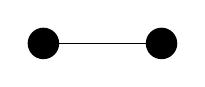
\begin{tikzpicture}
        \fill [black] (0,0) circle (0.2 cm);
        \draw (0,0) -- node {\midarrow} (1.5,0);
        \fill[black] (1.5,0) circle (0.2cm);
        \end{tikzpicture}
    \end{gathered}+
    \begin{gathered}
        \begin{tikzpicture}
        \fill [black] (0,0) circle (0.2 cm);
        \draw (0,0) -- (1.5,0);
        \fill[black] (1.5,0) circle (0.2cm);
        \draw (0.75,0.25) circle (0.25 cm);
        \draw[-triangle 90] (0.4,0) -- (0.41,0);
        \draw[-triangle 90] (1.15,0) -- (1.16,0);
        \draw[-triangle 90] (0.75,0.5) -- (0.76,0.5);
        \end{tikzpicture}
    \end{gathered}+
    \begin{gathered}
        \begin{tikzpicture}
        \fill [black] (0,0) circle (0.2 cm);
        \draw (0,0) -- (1.5,0);
        \fill[black] (1.5,0) circle (0.2cm);
        \draw (0.75,0.25) circle (0.25 cm);
        \draw (0.75,0.75) circle (0.25 cm);
        \draw[-triangle 90] (0.4,0) -- (0.41,0);
        \draw[-triangle 90] (1.15,0) -- (1.16,0);
        \draw[-triangle 90] (0.95,0.25) -- (0.95,0.24);
        \draw[-triangle 90] (0.95,0.6) -- (0.95,0.59);
        \end{tikzpicture}
    \end{gathered}+
    \begin{gathered}
        \begin{tikzpicture}
        \fill [black] (0,0) circle (0.2 cm);
        \draw (0,0) -- (2,0);
        \fill[black] (2,0) circle (0.2cm);
        \draw (1,0) circle (0.4 cm);
        \draw[-triangle 90] (0.4,0) -- (0.41,0);
        \draw[-triangle 90] (1.7,0) -- (1.71,0);
        \draw[-triangle 90] (1.,0) -- (1.01,0);
        \draw[-triangle 90] (1.,0.4) -- (1.01,0.4);
        \draw[-triangle 90] (1.,-0.4) -- (0.9,-0.4);
        \end{tikzpicture}
    \end{gathered}\\
    &+\begin{gathered}
        \begin{tikzpicture}
        \fill [black] (0,0) circle (0.2 cm);
        \draw (0,0) -- (3,0);
        \fill[black] (3,0) circle (0.2cm);
        \draw (1,0.25) circle (0.25 cm);
        \draw (2,0.25) circle (0.25 cm);
        \draw[-triangle 90] (0.5,0)--(0.51,0);
        \draw[-triangle 90] (1.5,0)--(1.51,0);
        \draw[-triangle 90] (2.5,0)--(2.51,0);
        \draw[-triangle 90] (1,0.5)--(1.01,0.5);
        \draw[-triangle 90] (2,0.5)--(2.01,0.5);
        \end{tikzpicture}
    \end{gathered}+
    \begin{gathered}
        \begin{tikzpicture}
        \fill [black] (-0.5,-0.5) circle (0.2 cm);
        \fill [black] (-0.5,0.5) circle (0.2 cm);
        \fill [black] (0.5,0.5) circle (0.2 cm);
        \fill [black] (0.5,-0.5) circle (0.2 cm);
        \draw (-0.5,-0.5) -- (0.5,0.5);
        \draw (-0.5,0.5) -- (0.5,-0.5);
        \draw[-triangle 90] (0.25,0.25)--(0.26,0.26);
        \draw[-triangle 90] (-0.16,0.15)--(-0.15,0.14);
        \draw[-triangle 90] (-0.16,-0.15)--(-0.15,-0.14);
        \draw[-triangle 90] (0.15,-0.15)--(0.25,-0.25);
        \end{tikzpicture}
    \end{gathered}+
    \begin{gathered}
        \begin{tikzpicture}
        \fill [black] (-0.7,-0.7) circle (0.2 cm);
        \fill [black] (-0.7,0.7) circle (0.2 cm);
        \fill [black] (0.7,0.7) circle (0.2 cm);
        \fill [black] (0.7,-0.7) circle (0.2 cm);
        \draw (0,0) circle (0.25 cm);
        \draw (-0.7,-0.7) -- (-0.25,0);
        \draw (-0.7,0.7) -- (-0.25,0);
        \draw (0.7,0.7) -- (0.25,0);
        \draw (0.7,-0.7) -- (0.25,0);
        \draw[-triangle 90] (-0.5,0.4)--(-0.4,0.3);
        \draw[-triangle 90] (-0.5,-0.4)--(-0.4,-0.3);
        \draw[-triangle 90] (0.4,0.3)--(0.5,0.4);
        \draw[-triangle 90] (0.4,-0.3)--(0.5,-0.4);
        \draw[-triangle 90] (0,0.25) -- (0.1,0.25);
        \draw[-triangle 90] (0,-0.25) -- (0.1,-0.25);
        \end{tikzpicture}
    \end{gathered}+
        \begin{gathered}
        \begin{tikzpicture}
        \fill [black] (-0.7,-0.7) circle (0.2 cm);
        \fill [black] (-0.7,0.7) circle (0.2 cm);
        \fill [black] (0.7,0.7) circle (0.2 cm);
        \fill [black] (0.7,-0.7) circle (0.2 cm);
        \draw (0,0) circle (0.25 cm);
        \draw (-0.7,-0.7) -- (-0.25,0);
        \draw (-0.7,0.7) -- (-0.25,0);
        \draw (0.7,0.7) -- (0.25,0);
        \draw (0.7,-0.7) -- (0.25,0);
        \draw[-triangle 90] (-0.4,0.3)--(-0.5,0.4);
        \draw[-triangle 90] (-0.5,-0.4)--(-0.4,-0.3);
        \draw[-triangle 90] (0.5,0.4)--(0.4,0.3);
        \draw[-triangle 90] (0.4,-0.3)--(0.5,-0.4);
        \draw[-triangle 90] (0,0.25) -- (0.1,0.25);
        \draw[-triangle 90] (0,-0.25) -- (-0.1,-0.25);
        \end{tikzpicture}
    \end{gathered}+\\
    &\begin{gathered}
        \begin{tikzpicture}
        \fill [black] (-0.5,-0.5) circle (0.2 cm);
        \fill [black] (-0.5,0.5) circle (0.2 cm);
        \fill [black] (0.8,0.8) circle (0.2 cm);
        \fill [black] (0.5,-0.5) circle (0.2 cm);
        \draw (-0.5,-0.5) -- (0.8,0.8);
        \draw (-0.5,0.5) -- (0.5,-0.5);
        \draw (0.6,0.3) circle (0.2 cm);
        \draw[-triangle 90] (0.25,0.25)--(0.26,0.26);
        \draw[-triangle 90] (-0.16,0.15)--(-0.15,0.14);
        \draw[-triangle 90] (-0.16,-0.15)--(-0.15,-0.14);
        \draw[-triangle 90] (0.15,-0.15)--(0.25,-0.25); 
        \draw[-triangle 90] (0.7,0.1)--(0.8,0.2); 
        \end{tikzpicture}
    \end{gathered}
    +\begin{gathered}
        \begin{tikzpicture}
        \fill [black] (-0.5,-0.5) circle (0.2 cm);
        \fill [black] (-0.5,0.5) circle (0.2 cm);
        \fill [black] (0.8,0.8) circle (0.2 cm);
        \fill [black] (0.5,-0.5) circle (0.2 cm);
        \draw (-0.5,-0.5) -- (0.8,0.8);
        \draw (-0.5,0.5) -- (0.5,-0.5);
        \draw (0.6,0.3) circle (0.2 cm);
        \draw[-triangle 90] (0.25,0.25)--(0.26,0.26);
        \draw[-triangle 90] (-0.16,0.15)--(-0.15,0.14);
        \draw[-triangle 90] (-0.16,-0.15)--(-0.15,-0.14);
        \draw[-triangle 90] (0.15,-0.15)--(0.25,-0.25); 
        \draw[-triangle 90] (0.8,0.2)--(0.7,0.1); 
        \end{tikzpicture}
    \end{gathered}+\order{\lambda^3}
    \end{aligned}
    \label{W_phi4_complex}
\end{equation}